\documentclass[11pt]{article}

\usepackage[margin=1in]{geometry}
\usepackage[T1]{fontenc}
\usepackage{lmodern}
\usepackage{fontspec}
\setmainfont{Calibri}
\usepackage{amsmath,amssymb}
\usepackage{graphicx}
\usepackage{enumitem}
\usepackage{url}
\usepackage[strings]{underscore}
\usepackage[hidelinks]{hyperref}

\newcommand{\gmfig}[2]{%
  \IfFileExists{gruggle_testsuite/#1.pdf}{\includegraphics[width=#2]{gruggle_testsuite/#1.pdf}}{%
    \texttt{[Missing PDF figure gruggle\_testsuite/#1.pdf]}}}

\title{Greggle \& Gruggle: Composable Regular Path Queries and Graph Manipulation}
\author{Sambuddha Majumder, Jayanta Majumder, Partha P Chakrabarti}
\date{\today}

\begin{document}
\maketitle

\begin{abstract}
Greggle is a small query language and tool for performing regular path queries over labelled directed graphs. Gruggle is a companion Node.js utility for ingesting, merging, inspecting, and lightly manipulating graphs in the Graphviz \texttt{dot} format. Graphviz is a widely used system for graph visualization; its \texttt{dot} language is simple to author and makes it easy to view results with standard Graphviz tools. Together the two utilities provide a frictionless workflow: Gruggle builds, merges, filters, and styles graphs; Greggle answers expressive path queries with edge-level predicates; and Gruggle can consume Greggle's annotations (e.g., \texttt{find-path}) to visualize witnesses. This document presents both tools, why they are complementary, and how they can be used jointly in analysis and visualization tasks.
\end{abstract}

\section{Introduction}

Many applications, from network analysis and access-control policy checking to program analysis and model checking, involve reasoning about paths in a labelled directed graph. In such settings one often cares not merely about reachability, but about the \emph{sequence of labels} seen along a path. Regular path queries provide a natural way to express such conditions.

Greggle is a lightweight system for expressing and evaluating such queries. Queries are S-expressions that combine regular expressions over edge labels with logical connectives (AND, OR, NOT) and existential quantification over node variables. A particular emphasis of Greggle is on \emph{edge-level predicates}: small boolean formulas over labels that must hold on individual edges, integrated into the regular expressions. Internally, query evaluation is performed using BDD-backed finite-domain relations \cite{bryant1986graph}, but this document focuses on surface behaviour and usage. The automata-based path interrogation approach follows classical constructions \cite{vardi2007automata}.

Gruggle is a small Node.js tool for ingesting, merging, inspecting, and lightly manipulating graphs in the Graphviz \texttt{dot} format from the command line. It combines a permissive \texttt{dot} parser with a composable subcommand pipeline that can add nodes, add edges (optionally random), prune isolated nodes, perform path-based keep/remove filtering, and export to SVG via Graphviz \texttt{dot}.

Together, Gruggle provides practical graph construction, merging, selection, and visualization; Greggle provides formal path-query answering. Gruggle can call Greggle's \texttt{find-path} to mark a witness path with a label, and Greggle can operate on Gruggle-produced dot files. The combined workflow lets you script graph edits, run precise path queries, and visualize results, all with small, dependency-light tools.

\section{Toolchain Overview}

\begin{itemize}[leftmargin=*]
  \item \textbf{Build and shape graphs with Gruggle.} Parse and merge {\em dot} formatted graphs, add synthetic structure (chains, rings, grids, cliques), delete or filter nodes/edges, and style elements.
  \item \textbf{Ask path questions with Greggle.} Express regular-path conditions with edge predicates (\texttt{all-of}, \texttt{some-of}, \texttt{negate}) and logical composition over node variables.
  \item \textbf{Visualize and iterate.} Use Gruggle to emit SVGs of intermediate or final graphs. Invoke \texttt{find-path} to have Greggle annotate one matching path for inspection.
  \item \textbf{Directed analytics.} Gruggle offers indegree/outdegree selection; Greggle specialises in directed labelled paths, together covering common directed-graph tasks such as traffic-flow analysis or policy auditing.
\end{itemize}

\section{Greggle: Regular Path Queries with Edge Predicates}

We now include the Greggle specification, highlighting how it can consume dot formatted graphs (including those shaped by Gruggle) and how its \texttt{find-path} output can be re-imported into Gruggle for visualization.

\subsection{Graphs}
\label{sectionOnGraphs}
A graph is a finite labelled directed graph $G = (V,E)$, where $V$ is a set of nodes and $E \subseteq V \times 2^{\Sigma} \times V$ is a set of edges. Each edge $(u,L,v)$ goes from node $u$ to node $v$ and carries a finite set of labels $L \subseteq \Sigma$ from a fixed alphabet of strings $\Sigma$.

In our prototype implementation and examples we often use Graphviz dot snippets to describe graphs, but the paradigm applies equally well to any in-memory labelled graph structure or object model. For example Figure \ref{fig:neg_demo} defines a graph with three nodes and three labelled edges. The dot parser supports multi-labelled edges by allowing comma-separated labels in the attribute value, e.g.\ \texttt{label="a,b"} denotes $L = \{\texttt{a},\texttt{b}\}$.

\begin{figure}[h]
  \centering
  \begin{minipage}{0.45\textwidth}
    \centering
    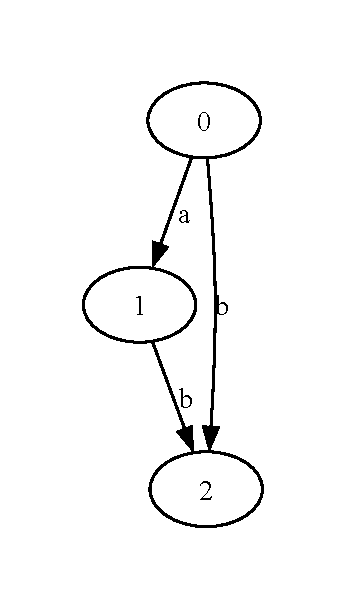
\includegraphics[width=0.5\linewidth]{testsuite/neg_demo} 
  \end{minipage}
  \hfill
  \begin{minipage}{0.45\textwidth}
\begin{verbatim}
digraph neg_demo {
  0;
  1;
  2;
  0 -> 1 [label="a"];
  0 -> 2 [label="b"];
  1 -> 2 [label="b"];
}
\end{verbatim}
\end{minipage}  
\caption{An edge-labelled graph and its dot format specification}
\label{fig:neg_demo}
\end{figure}

\subsection{Edge Predicates}

At the heart of Greggle's regular expressions are \emph{edge-level predicates}. Intuitively, an edge predicate $P$ is a boolean expression that can be evaluated on the label set $L$ of a single edge, yielding true or false. Greggle provides the following primitive constructors:
\begin{itemize}[leftmargin=*]
  \item Atomic label test: \texttt{a} is true on an edge whose label set contains the symbol \texttt{a}.
  \item Wildcard: \texttt{dot} is true on every edge, regardless of its label set (analogous to ``.'' in traditional regular expressions).
  \item Source-node lift: \texttt{P@} is true on an edge when the string regular expression \texttt{P} matches the label of the source node of that edge.
  \item Sink-node lift: \texttt{@P} is true on an edge when the string regular expression \texttt{P} matches the label of the sink node of that edge.
  \item Negation: \texttt{(negate $P$)} is true when $P$ is false on that edge.
  \item All-of: \texttt{(all-of $P_1$ $P_2$ $\dots$)} is true when each $P_i$ is true on that edge.
  \item Some-of: \texttt{(some-of $P_1$ $P_2$ $\dots$)} is true when at least one $P_i$ is true on that edge.
\end{itemize}
These constructors can be nested arbitrarily. As convenient shorthand, a leading tilde on an atom is interpreted as negation, so \texttt{\textasciitilde a} is equivalent to \texttt{(negate a)}.

For example:
\begin{itemize}[leftmargin=*]
  \item \texttt{a} holds on an edge with labels $\{\texttt{a},\texttt{b}\}$; \texttt{\textasciitilde a} does not.
  \item \texttt{(all-of a b)} holds on an edge with labels $\{\texttt{a},\texttt{b}\}$ but not on one with just $\{\texttt{a}\}$.
  \item \texttt{(some-of b c)} holds on an edge with labels $\{\texttt{b},\texttt{c}\}$ and also on one with labels $\{\texttt{b}\}$ or $\{\texttt{c}\}$.
  \item \texttt{MID@} holds on an edge whose source node label matches the regex \texttt{MID}.
  \item \texttt{@TARGET} holds on an edge whose sink node label matches the regex \texttt{TARGET}.
\end{itemize}

\subsection{Path Expressions}

Path expressions describe sets of finite paths in the graph. They are regular expressions whose atomic symbols are edge predicates. The syntax is:
\begin{itemize}[leftmargin=*]
  \item \texttt{P}, where $P$ is an edge predicate, denotes a single edge on which $P$ holds.
  \item \texttt{(concat $r_1$ $r_2$ $\dots$ $r_n$)} denotes concatenation: paths formed by following a subpath in $r_1$, then $r_2$, etc.
  \item \texttt{(alt $r_1$ $r_2$ $\dots$ $r_n$)} denotes alternation: a path is accepted if it is accepted by some $r_i$.
  \item \texttt{(star $r$)} denotes Kleene star, any finite concatenation of paths in the language of $r$ (including the empty path).
  \item \texttt{(plus $r$)} denotes one-or-more repetitions of $r$.
\end{itemize}

In practice, an atomic symbol \texttt{a} is treated as the edge predicate testing for label \texttt{a}, and we omit the explicit \texttt{sym} constructor sometimes found in other presentations.

\subsection{Query Expressions}

Building on path expressions, Greggle defines expressions that relate node variables:
\begin{itemize}[leftmargin=*]
  \item \texttt{(exists-path x y $r$)} is true under an assignment of nodes to variables $x$ and $y$ when there exists a path from $x$ to $y$ in the graph whose sequence of edge labels is accepted by the path expression $r$.
  \item \texttt{(match x $p$)} is true when the label of node $x$ matches the string regular expression $p$ in the usual sense of \texttt{std::regex\_match}.
  \item \texttt{(no-edge x y)} is true when there is \emph{no} edge from $x$ to $y$ in the graph.
  \item \texttt{(no-connection x y)} is true when there is no edge between $x$ and $y$ in either direction (neither $x \to y$ nor $y \to x$).
  \item \texttt{(same x y)} is true when $x$ and $y$ are assigned the same node.
  \item \texttt{(different x y)} is true when $x$ and $y$ are assigned different nodes.
  \item \texttt{(and $e_1$ $e_2$ $\dots$ $e_n$)} is true when all subexpressions are true under the current assignment.
  \item \texttt{(or $e_1$ $e_2$ $\dots$ $e_n$)} is true when at least one $e_i$ is true.
  \item \texttt{(not $e$)} is the logical complement.
  \item \texttt{(exists (x y $\dots$) $e$)} existentially quantifies over the listed variables, projecting them out of the final result.
\end{itemize}

The free variables of an expression are those that are not bound by an enclosing \texttt{exists}. Evaluating a query on a fixed graph yields a relation over the free variables; the query tool displays this as a set of satisfying bindings.

\section{Informal Semantics}

\subsection{Path Semantics}

Path expressions are interpreted as sets of paths over labelled edges. For \texttt{exists-path}, this induces a binary relation over nodes: $(u,v)$ is in the relation when there is a path from $u$ to $v$ whose label-sequence is accepted by the path expression. Alternation yields union of relations, concatenation yields relational composition, star yields reflexive-transitive closure, and plus yields transitive closure.

\subsection{Expression Semantics}

Queries over variables compose relations using standard boolean and relational connectives. For example, \texttt{(and (exists-path x y r1) (exists-path y z r2))} denotes the set of triples $(x,y,z)$ where both relations hold. Projection via \texttt{exists} removes bound variables from the reported relation; \texttt{not} and the binary absence tests allow expressing negative conditions (e.g., ``no edge between \texttt{x} and \texttt{y}'').

\section{Implementation Sketch}

The implementation follows the usual automata-based approach to regular path queries but adds an explicit predicate evaluator on edges and a symbolic relation layer:
\begin{enumerate}[leftmargin=*]
  \item \textbf{NFA construction:} Each path expression is compiled to an NFA with predicate-labelled transitions; concatenation, alternation, star, and plus are handled via epsilon-transitions in the standard way.
  \item \textbf{Product search:} For \texttt{exists-path}, the NFA is run over the graph by BFS over pairs of (graph node, NFA state), enabling transitions when the edge predicate holds on the edge's label set.
  \item \textbf{Relational composition:} The relations produced by \texttt{exists-path} are combined using relational operators (intersection, union, projection, complement), implemented symbolically using BDD-backed finite-domain relations.
\end{enumerate}

\subsection*{Path Evaluation via NFA}

Each path expression is compiled into a small NFA. States are classified as accepting or non-accepting, and transitions are labelled either by edge predicates (for consuming one edge) or by epsilon-transitions (for moving between states without consuming an edge). Regular expression constructs are handled in the standard way:
\begin{itemize}[leftmargin=*]
  \item A symbol (edge predicate) becomes a two-state NFA with a single consuming transition.
  \item Concatenation connects the end states of each component using epsilon-transitions.
  \item Alternation introduces a fresh start and end state and connects them via epsilon-transitions to and from each component.
  \item Star and plus introduce loops via epsilon-transitions to allow repeated traversal.
\end{itemize}

To evaluate \texttt{(exists-path x y $r$)} on a graph $G$, the system runs a breadth-first search over pairs $(u,q)$ where $u$ is a graph node and $q$ is an NFA state. For each start node $s$, the search is initialized at all NFA states reachable from the NFA start by epsilon-transitions, paired with $s$. The algorithm repeatedly:
\begin{itemize}[leftmargin=*]
  \item Dequeues a pair $(u,q)$.
  \item If $q$ is accepting, records $(x=u,y=u')$ as satisfying, where $u'$ is the current node in that pair.
  \item For each outgoing edge $(u,L,v)$ in $G$ and each NFA transition from $q$ labelled by edge predicate $P$, checks whether $P$ holds on the label set $L$. If so, it follows that transition to a new NFA state $q'$, computes the epsilon-closure of $q'$, and enqueues any new pairs $(v,q'')$ not seen before.
\end{itemize}

The result of this search is a set of node pairs $(s,t)$ that constitute the relation for \texttt{exists-path} over the variables $(x,y)$.

\subsection*{Symbolic Relations with BDDs}

Relations over node variables are represented symbolically using a finite-domain BDD layer. Each logical variable is associated with a finite-domain identifier; the underlying BDD package provides operations to represent and manipulate finite-domain predicates over these identifiers. A relation is thus encoded as a BDD whose variables correspond to the finite-domain variables for the logical variables.

Given a tuple of node values $(v_1,\dots,v_k)$ over variables $(x_1,\dots,x_k)$, the system constructs a conjunction of finite-domain predicates stating that each variable $x_i$ equals value $v_i$, and ORs these into the BDD representing the relation. From this representation, the following relational operations are implemented:
\begin{itemize}[leftmargin=*]
  \item \textbf{Union} and \textbf{Intersection} via BDD disjunction and conjunction, respectively.
  \item \textbf{Set difference} by conjunction with the negation of the other relation.
  \item \textbf{Projection} by existential quantification over the finite-domain variables corresponding to quantified logical variables.
  \item \textbf{Complement} by BDD negation, with respect to the full product domain of the participating variables.
\end{itemize}

\subsection*{Edge Predicate Evaluation}

Edge predicates are represented as small trees with nodes for atomic tests and boolean connectives (negation, all-of, some-of). Each atomic test stores a label name. Evaluation of a predicate $P$ on an edge is implemented by recursively traversing this tree:
\begin{itemize}[leftmargin=*]
  \item An atomic predicate compares its label name to the edge's label set.
  \item A negation node inverts the result of its child.
  \item An all-of node checks that all child predicates hold.
  \item A some-of node checks that at least one child predicate holds.
\end{itemize}

During NFA traversal, these predicates are used to decide which transitions are enabled on a given edge. This design cleanly separates path structure (handled by the NFA) from local label conditions (handled by predicate evaluation).

\subsection*{Query Tool Pipeline}

The command-line query tool ties these pieces together:
\begin{enumerate}[leftmargin=*]
  \item Parses a dot snippet or other graph description into the internal graph structure.
  \item Parses the query S-expression into the expression and path ASTs, including edge predicates.
  \item Evaluates the expression on the graph, constructing and combining symbolic relations as needed.
  \item Traverses the resulting relation and prints each satisfying binding, mapping internal node indices back to external node identifiers where appropriate.
\end{enumerate}

This architecture allows Greggle to support expressive regular path queries with edge-level predicates while keeping the implementation modular: path processing is localized to the NFA construction and product search, whereas relational composition and quantification are handled uniformly by the BDD-backed finite-domain layer.

\section{Examples}

\subsection{An Example Graph}

Figure~\ref{fig:handmade-sample} shows an example graph with mixed labels, illustrating the style of graphs Greggle is designed to work with. Nodes represent network states, edges represent transitions labelled by actions or propositions.

\begin{figure}[t]
  \centering
  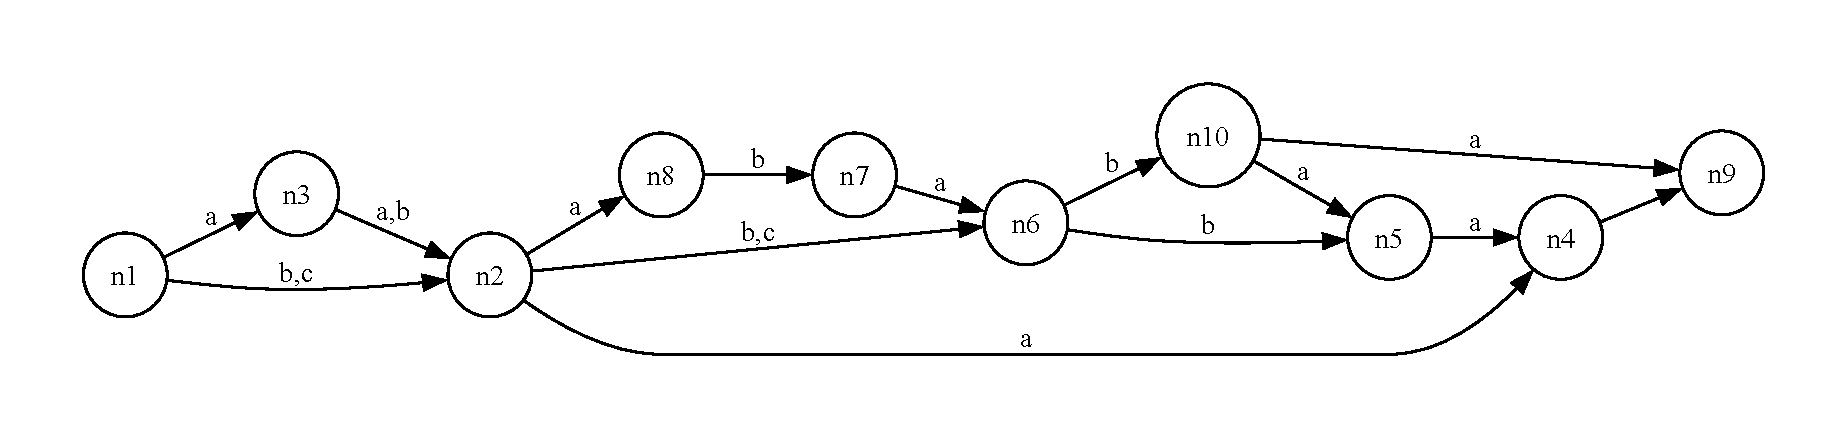
\includegraphics[width=\textwidth]{testsuite/handmade_sample.pdf}
  \caption{Example labelled graph used in several path queries.}
  \label{fig:handmade-sample}
\end{figure}

On this graph, one can express queries such as:
\begin{itemize}[leftmargin=*]
  \item Paths starting with \texttt{a} and then repeating \texttt{b\,a} one or more times:
\begin{verbatim}
(exists-path x y (concat a (plus (concat b a))))
\end{verbatim}
  \item Pairs of nodes connected by a path of only \texttt{c}-edges and also by a path matching the previous pattern:
\begin{verbatim}
(and (exists-path x y (star c))
     (exists-path x y (concat a (plus (concat b a)))))
\end{verbatim}
\end{itemize}
These examples exercise nested regular expressions and relational conjunction.

\subsection{Negated Edge Predicate}

Consider again the small graph \texttt{neg\_demo} mentioned in Section~\ref{sectionOnGraphs}. The query
\begin{verbatim}
(exists-path x y ~a)
\end{verbatim}
asks for all pairs $(x,y)$ such that there exists a single edge from $x$ to $y$ whose label set does not contain \texttt{a}. On this graph, the satisfying bindings are:
\begin{verbatim}
Satisfying bindings:
x=0 y=2
x=1 y=2
\end{verbatim}
corresponding exactly to the two edges labelled \texttt{b}.

\subsection{All-of and Some-of}

Now consider the graph in Figure \ref{fig:all_some_demo}.
\begin{figure}[h]
  \centering
  \begin{minipage}{0.45\textwidth}
\begin{verbatim}
digraph all_some_demo {
  0;
  1;
  2;
  0 -> 1 [label="a,b"];
  0 -> 2 [label="a"];
  1 -> 2 [label="b,c"];
}
\end{verbatim}
  \end{minipage}\hfill
  \begin{minipage}{0.45\textwidth}
    \centering
    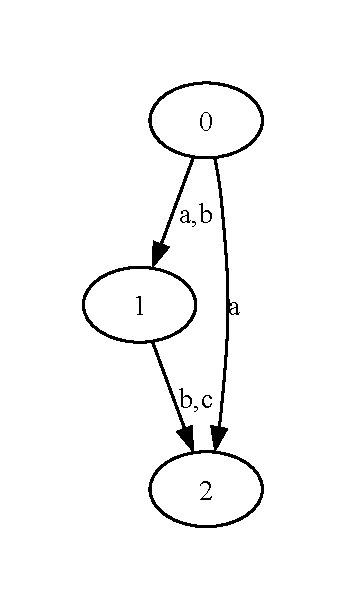
\includegraphics[width=0.5\linewidth]{testsuite/all_some_demo.pdf} 
  \end{minipage}
  \caption{A graph with multi-labelled edges}
    \label{fig:all_some_demo}
\end{figure}

The query
\begin{verbatim}
(exists-path x y (all-of a b))
\end{verbatim}
asks for all edges that have both labels \texttt{a} and \texttt{b}. On this graph, the only such edge is $0 \to 1$, and the result is:
\begin{verbatim}
Satisfying bindings:
x=0 y=1
\end{verbatim}

The query
\begin{verbatim}
(exists-path x y (some-of b c))
\end{verbatim}
asks for all edges that have \texttt{b} or \texttt{c} (or both). Here both $0\to 1$ and $1\to 2$ satisfy this predicate, yielding:
\begin{verbatim}
Satisfying bindings:
x=0 y=1
x=1 y=2
\end{verbatim}
These examples demonstrate how edge-level predicates express conditions involving the presence or absence of multiple labels on a single edge.

\subsection{Wildcard and Relational Predicates}

The \texttt{dot} predicate acts as a wildcard edge test: it is true on every edge, regardless of its label set. On the graph \texttt{neg\_demo} from Section~\ref{sectionOnGraphs}, the query
\begin{verbatim}
(exists-path x y dot)
\end{verbatim}
asks for all single-edge connections in the graph, and yields exactly the set of edges:
\begin{verbatim}
Satisfying bindings:
x=0 y=1
x=0 y=2
x=1 y=2
\end{verbatim}

The predicate \texttt{(no-edge x y)} expresses the absence of a directed edge from $x$ to $y$, while \texttt{(no-connection x y)} expresses the absence of any edge between $x$ and $y$ in either direction. On \texttt{neg\_demo}, for example, \texttt{(no-connection x y)} holds only when $x$ and $y$ are the same node, since every unordered pair of distinct nodes is joined by at least one edge.

Finally, the predicates \texttt{(same x y)} and \texttt{(different x y)} implement equality and inequality over node variables. On a graph with nodes $0,1,2$, \texttt{(same x y)} yields bindings \texttt{x=0,y=0}, \texttt{x=1,y=1}, \texttt{x=2,y=2}, while \texttt{(different x y)} yields all pairs where the node components are distinct. These relational primitives make it easy to combine path-based conditions with simple structural constraints on node assignments.

Node-label tests can also be lifted into edge predicates inside a path expression. If \texttt{P} is a string regular expression over node labels, then \texttt{P@} tests the source node of the edge and \texttt{@P} tests the sink node. For instance,
\begin{verbatim}
(exists-path x y (all-of a @TARGET))
\end{verbatim}
matches \texttt{a}-labelled edges whose sink node label matches \texttt{TARGET}, while
\begin{verbatim}
(exists-path x y (all-of a MID@))
\end{verbatim}
matches \texttt{a}-labelled edges whose source node label matches \texttt{MID}. Since these are ordinary edge predicates, they compose normally with \texttt{negate}, \texttt{all-of}, and \texttt{some-of}.

As a final illustration, consider a graph whose node labels are strings such as \texttt{A}, \texttt{AB}, \texttt{B1}, \texttt{Z}, with edges labelled by atomic propositions \texttt{a}, \texttt{b}. The query
\begin{verbatim}
(and (match x "A.*")
     (exists-path x y a))
\end{verbatim}
asks for all pairs $(x,y)$ such that the label of $x$ matches the pattern \texttt{A.*} and there is an edge labelled \texttt{a} from $x$ to $y$. On a graph where there is an \texttt{a}-edge from \texttt{A} to \texttt{Z} but only a \texttt{b}-edge from \texttt{AB} to \texttt{Z}, the only satisfying binding is \texttt{x=A,y=Z}, combining a label-based filter with a path predicate.

\section{DOT-Based Query Tool}

The Greggle query tool is a command-line program that takes a Graphviz dot file and a query expression as arguments, and prints the satisfying bindings. Its usage is:
\begin{verbatim}
greggle <graph.dot> "<query in lisp syntax>"
\end{verbatim}
where the query must be quoted so that it is passed as a single argument.

Internally, the tool:
\begin{enumerate}[leftmargin=*]
  \item Parses the Graphviz dot file, assigning each node identifier a unique integer index and collecting edge label sets.
  \item Parses the query S-expression, building the abstract syntax tree for path and edge predicates.
  \item Evaluates the query on the graph to obtain a relation over the free variables.
  \item Prints each satisfying binding as a line of the form \texttt{x=nodeLabel y=nodeLabel}, mapping internal node indices back to the original Graphviz dot labels.
\end{enumerate}

For example, running the tool on \texttt{neg\_demo.dot} with the negated edge predicate query produces:
\begin{verbatim}
Satisfying bindings:
x=0 y=2
x=1 y=2
\end{verbatim}
matching the hand analysis above.

\section{Future Work}

Possible extensions include incorporating richer node/edge attributes into predicates, adding shortest-path variants of regular path queries, supporting incremental updates for dynamic graphs, and tighter integration with visualization (e.g., highlighting all satisfying paths, not just one witness).

\section{Gruggle: Graphviz Graph Manipulation and Visualization}

\subsection{Command Line and Entry Point}

The main executable is \texttt{gruggle.js}. It accepts zero or more input files using repeated \texttt{-i} flags. All parsed graphs are merged; if no inputs are given an empty digraph is used. Style switches: \texttt{--curved} (default) for curved spline edges, \texttt{--ortho} or \texttt{--rectilinear} for rectilinear edges (\texttt{splines=ortho}). After parsing/merging, subcommands are applied in order. Examples:
\begin{verbatim}
node gruggle.js --ortho -i g1.dot -i g2.dot set-name merged to-svg merged.svg
node gruggle.js chain "add-node nx:1:100" "add-edge 50 nx.* nx.*" \
                     "keep-paths nx1 nx5" "to-svg pruned.svg"
\end{verbatim}

\subsection{Graphviz Dot-format Parsing and Merging}

The parser handles both \texttt{graph}/\texttt{digraph}, optional \texttt{strict}, named/unnamed graphs, subgraphs, edge ops \texttt{->}/\texttt{--}, port/compass points, bracketed attribute lists, quoted IDs, HTML-like IDs, numbers, comments (\texttt{//}, \texttt{/* */}, \texttt{\#}), and default attribute statements (\texttt{graph}, \texttt{node}, \texttt{edge}). When merging, later files' attributes override earlier ones on conflicts; edges are deduplicated by endpoints/ports/direction with attribute merge. Default emitted style: box-shaped, rounded, light-blue nodes and muted-blue edges; orthogonal vs.\ curved splines are controlled by the CLI switch above.

\subsection{Subcommands}

Subcommands operate on the in-memory graph and can be composed with the \texttt{chain} meta-command. Tokens inside a chain are parsed with a simple shell-like splitter (quotes supported).
\begin{itemize}[leftmargin=*]
  \item \textbf{set-name} \texttt{<name>}: rename the graph.
  \item \textbf{add-nodes} \texttt{<id>|<prefix:start:end>}: add a single node or a numeric range (e.g.\ \texttt{nx:1:3} $\rightarrow$ \texttt{nx1}, \texttt{nx2}, \texttt{nx3}).
  \item \textbf{add-edges} \texttt{<label> <fromRe> <toRe>}: add edges for all pairs whose IDs match the regexes, using the current graph direction. Attribute \texttt{label} is set when provided and non-empty.
  \item \textbf{add-edges} \texttt{<count> <fromRe> <toRe> [label]}: pick up to \texttt{count} random distinct pairs from the regex matches and add those edges (optional label).
  \item \textbf{add-chain} \texttt{<root> <n>}: add nodes \texttt{root\_1}.. \texttt{root\_n} linked in a chain.
  \item \textbf{add-grid} \texttt{<root> <rows> <cols>}: add a \texttt{rows} x \texttt{cols} grid with nodes \texttt{root\_i\_j} and directional grid edges (top-to-bottom, left-to-right).
  \item \textbf{delete-isolated-nodes}: remove nodes with no incident edges.
  \item \textbf{remove-nodes} \texttt{<regex>}: delete nodes matching the regex and their incident edges.
  \item \textbf{remove-edges-between-nodes} \texttt{<fromRe> <toRe>}: delete edges whose tail/head IDs match the regex pair.
  \item \textbf{add-labels-to-edges-on-paths} \texttt{<fromRe> <toRe> <label>}: add the given label on every edge lying on a path from sources matching \texttt{fromRe} to targets matching \texttt{toRe}.
  \item \textbf{remove-labels-from-edges-on-paths} \texttt{<fromRe> <toRe> <label>}: remove the given label from every edge lying on such paths; if no labels remain, the attribute is removed.
  \item \textbf{select-nodes} / \textbf{deselect-nodes} \texttt{<regex>}: mark/unmark nodes whose IDs match the regex.
  \item \textbf{select-edges} / \textbf{deselect-edges}: either \texttt{<labelRegex>} (matches any label component) or \texttt{<fromRe> <toRe>} (matches endpoints) to mark/unmark edges.
  \item \textbf{select-nodes-label} \texttt{<labelRegex>}: select nodes whose label attribute has a matching component.
  \item \textbf{delete-selected}: delete selected nodes (and their incident edges) and selected edges.
  \item \textbf{set-node-attr-on-selected} \texttt{<attr> <value>} / \textbf{set-edge-attr-on-selected} \texttt{<attr> <value>}: set a dot attribute on selected nodes/edges.
  \item \textbf{unset-node-attr-on-selected} \texttt{<attr>} / \textbf{unset-edge-attr-on-selected} \texttt{<attr>}: remove a dot attribute on selected nodes/edges.
  \item \textbf{clear-visual-attrs-on-selected}: clear common visual attributes (color, fillcolor, fontcolor, style, shape, penwidth, arrowsize, fontsize) on selected nodes/edges.
  \item \textbf{add-labels-to-selected} \texttt{<label>}: append the label (comma-separated) to all selected nodes and edges.
  \item \textbf{remove-labels-from-selected} \texttt{<label>}: remove the label from selected nodes/edges; drops the attribute if empty.
  \item \textbf{keep-paths} \texttt{<fromRe> <toRe>}: mark all nodes and edges that lie on at least one path from any source matching \texttt{fromRe} to any target matching \texttt{toRe}. Marks set \texttt{keep=true} and clear \texttt{remove}.
  \item \textbf{remove-paths} \texttt{<fromRe> <toRe>}: similarly mark nodes/edges on such paths, setting \texttt{remove=true} and clearing \texttt{keep}.
  \item \textbf{keep-path-edges} \texttt{<fromRe> <toRe>}: mark only the edges (not nodes) that lie on such paths with \texttt{keep=true}.
  \item \textbf{remove-path-edges} \texttt{<fromRe> <toRe>}: mark only the edges (not nodes) on such paths with \texttt{remove=true}.
  \item \textbf{filter-to-paths} \texttt{<fromRe> <toRe>}: keep only nodes/edges on such paths (mark all others as remove).
  \item \textbf{select-nodes-on-paths} \texttt{<fromRe> <toRe>}: select all nodes on such paths (for later bulk ops).
  \item \textbf{select-edges-on-paths} \texttt{<fromRe> <toRe>}: select all edges on such paths.
  \item \textbf{find-path} \texttt{<regex> <label>}: annotate one matching path's edges with the given label using Greggle-compatible regular-path semantics, including lifted node predicates such as \texttt{P@} and \texttt{@P}.
  \item \textbf{select-neighbours} \texttt{[in|out|both] <hops>}: expand selection by BFS over neighbours (default both,1).
  \item \textbf{select-nodes-degree} \texttt{<lt|le|eq|ge|gt> <k>}: select nodes by total degree (in+out for digraphs).
  \item \textbf{select-nodes-indegree} \texttt{<lt|le|eq|ge|gt> <k>}: select nodes by indegree (undirected edges count as both).
  \item \textbf{select-nodes-outdegree} \texttt{<lt|le|eq|ge|gt> <k>}: select nodes by outdegree (undirected edges count as both).
  \item \textbf{select-component-of-nodes} \texttt{<regex>}: select nodes/edges in components of matching nodes.
  \item \textbf{select-components-with-selected}: select nodes/edges in any component that already contains a selected node.
  \item \textbf{clear-selection}: clear selection on all nodes/edges.
  \item \textbf{invert-selection-nodes}: flip selection flags on nodes.
  \item \textbf{invert-selection-edges}: flip selection flags on edges.
  \item \textbf{chain} \texttt{"cmd1 ..."} \texttt{"cmd2 ..."}: run each nested command in order. Inside a chain, \texttt{-f <file>} splices commands line-by-line from the file (comments/blank lines skipped) at that point in sequence.
  \item \textbf{to-svg} \texttt{<filename>}: pipe the current graph through \texttt{dot -Tsvg -o <filename>} (assumes \texttt{dot} is on \texttt{PATH}).
\end{itemize}

\paragraph{Keep/remove semantics.}
Elements carry in-memory \emph{keep} and \emph{remove} flags that flip with the operations above (keep clears remove, remove clears keep). When emitting the final graph:
\begin{itemize}[leftmargin=*]
  \item If any element is marked keep, only kept elements are emitted.
  \item Otherwise, elements marked remove are suppressed; the rest are emitted.
\end{itemize}
No flags are written into dot attributes.

\subsection{Output}

Default output is dot on stdout, reflecting merged defaults and the current subcommand state. Using \texttt{to-svg} writes an SVG file via Graphviz with the same styling preamble (boxy light-blue nodes, blue edges, curved or orthogonal per CLI switch).

\subsection{Example Workflow}
\begin{verbatim}
# Merge two graphs, add 20 random edges among nx* nodes, retain only
# paths from nx1 to nx5, emit both dot and SVG with orthogonal edges.
node gruggle.js --ortho -i a.dot -i b.dot \
  chain "add-edge 20 nx.* nx.*" "keep-paths nx1 nx5" "to-svg pruned.svg" \
  > pruned.dot
\end{verbatim}

\subsection{Illustrative Examples}

\subsubsection{Ring/Chain/Grid Builders}
Figure~\ref{fig:chain-ring} and Figure~\ref{fig:grid} illustrate the synthetic builders discussed here.
\begin{figure}[h]
  \centering
  \gmfig{add_chain.golden}{0.4\textwidth}
  \gmfig{add_ring.golden}{0.4\textwidth}
  \caption{Left: chain of four nodes. Right: ring of three nodes.}
  \label{fig:chain-ring}
\end{figure}
\begin{figure}[h]
  \centering
  \gmfig{add_grid.golden}{0.5\textwidth}
  \caption{2x2 grid built with \texttt{add-grid g 2 2}.}
  \label{fig:grid}
\end{figure}
\begin{verbatim}
# Chain of four nodes c_1 -> c_2 -> c_3 -> c_4
node gruggle.js chain "add-chain c 4" > chain.dot

# Ring of three nodes r_0 -> r_1 -> r_2 -> r_0
node gruggle.js chain "add-ring r 3 0" > ring.dot

# 2x2 grid g_1_1, g_1_2, g_2_1, g_2_2 with edges down/right
node gruggle.js chain "add-grid g 2 2" > grid.dot
\end{verbatim}

\subsubsection{Random Selection and Labeling}
Figure~\ref{fig:rnd} shows random node/edge selection annotated with \texttt{rnd}.
\begin{figure}[h]
  \centering
  \gmfig{select_random_nodes_edges.golden}{0.45\textwidth}
  \caption{Randomly selected nodes/edges labeled \texttt{rnd}.}
  \label{fig:rnd}
\end{figure}
\begin{verbatim}
# Select up to 10 nodes and edges at random, mark them 'rnd'
node gruggle.js -i sample1.dot chain \
  "select-random-nodes 10 .*" \
  "select-random-edges 10 .* .*" \
  "add-labels-to-selected rnd" > random.dot
\end{verbatim}
Resulting edges/nodes carry labels like \texttt{name:rnd} or \texttt{label="x,rnd"}.

\subsubsection{Path Highlighting via Greggle (find-path)}
Figure~\ref{fig:pathlab} shows greggle-driven path annotation.
\begin{figure}[h]
  \centering
  \gmfig{find_path.golden}{0.5\textwidth}
  \caption{Edges on one matching path annotated with \texttt{pathlab}.}
   \label{fig:pathlab}
\end{figure}
\begin{verbatim}
# Highlight one path whose edge labels match (concat x y) with 'pathlab'
node gruggle.js -i sample1.dot chain \
  "find-path (concat x y) pathlab" > path_highlighted.dot
\end{verbatim}
Edges on the witness path gain \texttt{pathlab} in their label (e.g., \texttt{label="x,pathlab"}).

\subsubsection{Component-Based Selection}
Figure~\ref{fig:components} visualizes component selection from regex and from existing selection.
\begin{figure}[h]
  \centering
  \gmfig{select_component_of_nodes.golden}{0.45\textwidth}
  \gmfig{select_components_with_selected.golden}{0.45\textwidth}
  \caption{Selecting components by node regex (left) and from existing selection (right).}
  \label{fig:components}
\end{figure}
\begin{verbatim}
# Select components containing nodes matching x*
node gruggle.js -i comps.dot chain \
  "select-component-of-nodes x.*" \
  "add-labels-to-selected compA" > comps_marked.dot

# Select components containing already-selected nodes
node gruggle.js -i comps.dot chain \
  "select-nodes y2" \
  "select-components-with-selected" \
  "add-labels-to-selected compB" > comps2.dot
\end{verbatim}
Nodes and internal edges in those components are labeled \texttt{name:compA} or \texttt{name:compB}.

\subsubsection{Selection Utilities}
Figure~\ref{fig:visattrs} shows styling and clearing of selected elements.
\begin{figure}[h]
  \centering
  \gmfig{visual_attrs_on_selected.golden}{0.45\textwidth}
  \caption{Visual attrs set then cleared on selected nodes/edges.}
  \label{fig:visattrs}
\end{figure}
\begin{verbatim}
# Label-selected nodes/edges, then clear visual styling
node gruggle.js -i sample1.dot chain \
  "select-nodes s1" \
  "select-edges x" \
  "set-node-attr-on-selected fillcolor yellow" \
  "set-edge-attr-on-selected color red" \
  "clear-visual-attrs-on-selected" > styled.dot
\end{verbatim}

\subsubsection{Degree and Neighborhood Selection}
Figure~\ref{fig:deg-neigh} illustrates degree-based selection and neighbour expansion before the corresponding command snippets.
\begin{figure}[h]
  \centering
  \gmfig{select_nodes_degree.golden}{0.45\textwidth}
  \gmfig{select_neighbours.golden}{0.45\textwidth}
  \caption{Left: nodes with degree $\ge 3$ labeled \texttt{degsel}. Right: 2-hop neighbour expansion labeled \texttt{neigh}.}
  \label{fig:deg-neigh}
\end{figure}
\begin{verbatim}
# Select nodes with degree >= 3
node gruggle.js -i sample1.dot chain \
  "select-nodes-degree ge 3" \
  "add-labels-to-selected degsel" > deg.dot

# BFS expand selection by 2 hops (undirected sense)
node gruggle.js -i sample1.dot chain \
  "select-nodes s1" \
  "select-neighbours both 2" \
  "add-labels-to-selected neigh" > neigh.dot
\end{verbatim}

\subsubsection{Directed Indegree/Outdegree Selection}
Figure~\ref{fig:indeg-outdeg} shows indegree and outdegree filtering on a directed sample graph.
\begin{figure}[h]
  \centering
  \gmfig{select_nodes_indegree.golden}{0.45\textwidth}
  \gmfig{select_nodes_outdegree.golden}{0.45\textwidth}
  \caption{Left: nodes with indegree $\ge 2$ labeled \texttt{indegsel}. Right: nodes with outdegree $=0$ labeled \texttt{outdegsel}. Undirected edges count toward both in/out.}
  \label{fig:indeg-outdeg}
\end{figure}
\begin{verbatim}
# Indegree >= 2 (counts incoming arcs; undirected edges count as both)
node gruggle.js -i sample1.dot chain \
  "select-nodes-indegree ge 2" \
  "add-labels-to-selected indegsel" > indeg.dot

# Outdegree == 0 (no outgoing arcs; undirected edges count as both)
node gruggle.js -i sample1.dot chain \
  "select-nodes-outdegree eq 0" \
  "add-labels-to-selected outdegsel" > outdeg.dot
\end{verbatim}
These directed-aware predicates complement the total-degree selector when working with asymmetric graphs.

\section{Combined Use Cases}

\paragraph{Policy and reachability audits.} Use Gruggle to ingest firewall or service-topology dot, mark sources/targets, prune irrelevant nodes with \texttt{filter-to-paths}, then ask Greggle to find forbidden or required label sequences. Feed \texttt{find-path} results back into Gruggle to visualize witness or counterexample paths.

\paragraph{Dataflow debugging.} Build SSA or CFG fragments with Gruggle (\texttt{add-chain}, \texttt{add-grid}, \texttt{add-edges}), then use Greggle to assert sequences of operations (e.g., taint propagation) with edge predicates like \texttt{(all-of read taint)}. Visualize offending paths with Gruggle.

\paragraph{Interactive exploration.} Select dense regions with Gruggle's degree/indegree/outdegree selectors, expand neighbours, then run Greggle queries confined to those regions. This iterative loop narrows search space while preserving the ability to emit publication-ready diagrams.

\section{Conclusion}

Gruggle and Greggle form a lightweight, scriptable toolchain for labelled directed graphs: Gruggle for shaping, filtering, and rendering dot; Greggle for semantically rich regular path queries with edge predicates. Because both speak the dot format, they compose naturally: Gruggle prepares and visualizes; Greggle answers; Gruggle renders the answers. This combination supports quick exploratory analysis and repeatable pipelines without heavy dependencies.

\bibliographystyle{plain}
\bibliography{references}
\end{document}

